\documentclass[11pt,a4paper]{article}

\usepackage{color,graphicx,listings,wrapfig,hyperref,algpseudocode,algorithm}
%\usepackage[margin=2cm]{geometry}
\usepackage[toc,page]{appendix}
\usepackage{amsmath,subcaption}
\newcommand{\BigO}[1]{\ensuremath{\operatorname{O}\bigl(#1\bigr)}}

\graphicspath{{./img/}}

\begin{document}
\title{Second report from Threaded Programming}
\author{c02f-32d66e}
\maketitle

\section{Introduction}
\texttt{OpenMP} provides four basic schedulers that help parallel programs achieve the best performance. 
However, all of them are fairly simple and thus work optimally only in certain uncomplicated scenarios. 
As we show in the first report, a scheduler offering the best performance in all but the most simple cases is \texttt{dynamic}. 
While it is beneficial to use it, one might ask if it is possible to create another scheduler that would scale more efficiently with increasing (but moderate) number of processors. 
We show that it is indeed possible.

An implementation is presented in this report along with a detailed argument for its correctness and some discussion of reasons for the observed performance. The performance of this new scheduler, called \texttt{affinity} scheduler, is compared with the best scheduler for the same code determined in the first report. A brief comparison between different compilers is made and certain avenues for improvement are summarily suggested, but not investigated in depth.

\subsection{Definition of affinity scheduler}
The affinity scheduler tries to strike a balance between \texttt{dynamic} and \texttt{static} scheduling methods. 
It first divides the number of iterations evenly among processes and makes each process compute its own iterations first.
The number of iterations calculated every run of the scheduler is proportional to the number of iterations left in the pool of iterations.
Then once there are no iterations left in the current thread pool the thread ``steals'' iterations from the most loaded thread.
It is an improvement over the \texttt{dynamic} scheduler, as the overhead from thread synchronisation is omitted until later in the computation and on \texttt{static} as threads can share cycles between each other thus making computation in all but the simplest cases more efficient.

There are certain improvements to this scheduler that could be proposed almost immediately. For instance initially the workload could be divided between threads in a different proportion, which could help with some problems. 
Or the amount of iterations computed every scheduler run could be calculated in different way than inverse-proportionally to the number of iterations left in the pool.
Regardless of the possible improvements that could be made to the way the algorithm works, it was not our task to improve the affinity scheduler, and we will not develop these ideas further in this report nor in the code.

\section{Compiler, build system, style}
We have used the \texttt{gcc} compiler to compile the code we ran in parallel.
One could argue that it was not the best choice, as the Portland family of compilers offer performance that is even orders of magnitude better than what is provided by the \texttt{gcc}. 
This is correct, but we are limited in the compiler choice by the compiler we have chosen in the first report, which was \texttt{gcc}. 
Therefore when reading the performance results in the later parts of the report one must keep in mind that much better performance is readily possible by using a different compiler. 
Since what we aim for is a comparison between the built-in schedulers and affinity scheduler developed by us we needed to use the same compiler for the old and new runs giving us no other choice but to use \texttt{gcc}.

\subsection{Build system}
We considered using a different build system than just simple \texttt{GNU Make}, but we concluded it would not bring any benefit in this particular case. 
We don't need to have the code compilable under different architectures and compilers, it is enough to be able to compile it under Linux and \texttt{gcc}. 
Because of that \texttt{cmake} or \texttt{ant} would not bring any benefits to the compilation process adding unneeded dependencies. 

Makefiles have additional disadvantage though, which is their syntax. 
It can be in many cases confusing, impractical and lacking in many modern features many of developers are used to.
We feel that as much as it would be an issue in a bigger project, in our case of one file needing compilation these hurdles can be easily overcome.

\subsection{Style}
It is our preference to use the \href{https://www.kernel.org/doc/Documentation/CodingStyle}{Linux Kernel coding style}, with certain modifications. 
We feel that indenting by four spaces is more practical than eight-space indentation. 
We have also not modified the style of the parts of the code present before our modifications.
This can create a feeling of a certain disparity between these two code parts, but we think it fits more closely a real scenario where it is impractical (and possibly unwanted) to modify a big codebase which style is different from a coding style used for modifications.
Of course in a most optimal case all the projects should aim at would be to use a uniform style throughout the whole project.
In this situation though, we feel that such a style difference does not make the code less readable and is warranted.

We use \texttt{Doxygen}-compatible comments to describe function behaviour where appropriate. 
Routines to generate the actual documentation out of the source file were not provided, as they can be trivially added as needed.
We have not added comments to the code parts provided for the assignment that were not modified as this was not required.

\section{Implementation}
In the implementation of the affinity scheduler we preferred to use simpler solutions in places where more sophisticated ones would provide marginal performance benefits.
Such an approach has a marked benefit of simplifying the source thus making it less bug-prone and easier to comprehend.
Of course at certain places simpler algorithms have performance impact that cannot be tolerated.
We identified such bottlenecks, in most places, by routine profiler usage thus applying the optimisations with an evidence-based strategy.

\begin{algorithm}
    \caption{Affinity scheduler}\label{aff_src}
    \begin{algorithmic}[1]
        \State set up locks and chunk boundaries

        \While{1}
            \State set a lock on current threads' chunks
            \If{iterations available in current threads' pool}
                \State claim iterations
                \State release the lock on current threads' chunks
            \ElsIf{it is possible to ``steal'' iterations from a thread}
                \State release the lock on current threads' chunks
                \State set a lock on a most loaded threads' chunks
                \State claim iterations from a most loaded thread
                \State release lock on the most loaded threads' chunks
            \Else
                \State release lock on the current threads' chunks
                \State \textbf{break}
            \EndIf

            \If{iterations\_start = iterations\_end}
                \State \textbf{continue}
            \EndIf

            \State launch a correct loop
        \EndWhile
    \end{algorithmic}
\end{algorithm}

\subsection{Affinity scheduling algorithm dissection}
\subsubsection{Data structures used}
For keeping track of the iteration ranges left to be computed by different threads we use an array which has as many items as the number of threads. 
An entry in that array is a pair of numbers (wrapped in a \texttt{C} struct) that specify the beginning of the computation range and its end + 1. 
By keeping the first iteration that is not in the range assigned to the end value we make it more convenient to use this number in loops where one most commonly requires an iterator to be smaller than some threshold.
Checking for equality may lead to certain hard to find bugs\footnote{This is especially true with floating point numbers as equality checking in meaningless with them. It is less true with integer types used in this case, but it is a good habit to use ``less than'' instead of ``equals'' sign in loops.}.

There are other schemes that could be employed here. 
One could keep beginnings of a range in one array and the ends in another or not use a struct and remember that even indexes denote starts of a range and odd their ends. 
What all the other ways of keeping this data we considered have in common is making it harder to understand its meaning while reading and creating the program, and at the same time not providing any performance benefit.
Consequently, we decided to use the scheme described above for encapsulating the iteration ranges.

\paragraph{Data consistency}
Using just an array as described above is problematic when the same array is accessed by multiple threads.
Two writes occurring at the same time or a write happening with a read from another thread introduce a race condition that has to be avoided.
Main schemes that could be employed for dealing with this problem would be: performing reads and writes inside a critical section, using one lock for the whole array or using an array of locks for each element in the array.

The first two solutions are equivalent and share the same drawbacks. 
The overhead of essentially locking the whole array every time any read or write involving it is attempted would increase with a number of threads used, leading to a very unpleasant situation of threads spending a large part of their time waiting for array access.
Memory savings could be named as a reason to use a single lock, but even on severely memory-starved systems the size of multiple locks (four bytes per lock) would not be an impediment to implementation.

Because of the above considerations we used an array of locks, one lock corresponding to each process and thus the iteration range.
Care needs to be exercised while accessing the array of iteration ranges, as a proper lock needs to be set every time an iteration range is read from or written to.
Setting a lock before reading from the iteration ranges array (called \texttt{chunks} from now on) must happen as it is undesirable to have a write operation happening at the same time as a read.
Without locking \texttt{chunks} before a read it would be impossible to protect against this kind of a race condition.

\subsubsection{In-detail operation}
\paragraph{Initial setup}
This paragraph describes all the operations that happen at line 1 in Algorithm~\ref{aff_src}.
At first the \texttt{chunks} array and the corresponding locks arrays are allocated on the stack. 
Then the locks are initialized to be in an unset stage.
It is an important stage, without it the locks would be in undefined state with some parts of \texttt{chunks} permanently locked.

Then the parallel part begins with each thread setting its own chunk (iteration) boundaries without applying any locks.
Consistency of this operation is achieved though a \texttt{barrier} at the end of the chunk boundaries setting.
Thus no locks need setting as we have a guarantee that no two threads will try to write to or read from different parts of the \texttt{chunks} array.

\paragraph{Main scheduler loop}
It is described on the lines 2 -- 20 in Algorithm~\ref{aff_src}. 
The first condition, on line 4, depends on access to the \texttt{chunks} array and thus a lock on the array item containing its iteration ranges is needed before the condition is checked.
If there are any iterations left in the current threads' workload a proper amount of iterations is claimed and the lock is released.
If there are no iterations left local to the current thread, the iterations are ``stolen'' from the most loaded thread (lines 7 -- 11).
If there is any work left to be done in any of the threads ranges, the proper amount of iterations is claimed, with proper lock setting and releasing.
For the discussion on the operation of a method for determining the most loaded thread please see Section~\ref{sec:most_loaded}.
If there are no chunks to be ``stolen'' from any of the processes, it means that that there is no work this process can do and thus the main loop is stopped and the thread finishes execution.
Before that happens a lock on a current thread is released to prevent a deadlock.

If the scheduler continues for the current thread, a correct loop is launched.

\subsection{Finding a most loaded thread}
The function finding a most loaded thread iterates through the whole \texttt{chunks} array to determine a most loaded thread.
It does not use any kind of locking for two reasons. 
First of all, we wanted this function to have as small a performance impact as possible as it is launched fairly often in later parts of the computation for unbalanced loops, such as loop 2.
Using locking before each \texttt{chunks} read would hurt performance, substantially increasing computation time for higher processor counts.

Furthermore the only modifications possible to the chunks array after the initial initialization are increases of the starting point of each iteration range containing struct. 
This means that the only error that can be made by the function finding the most loaded thread is to point to a thread that was recently the most loaded thread. 
It has minimal effect on performance if this error is made, with the only difference being a slight divergence from the definition of an \texttt{affinity} scheduler.
Such a situation will occur rarely enough for us not to try to do everything possible to stop it.

The only case when this condition could have any effect on correctness of the result would be when there is only one iteration left, which is claimed by other thread before this function returns.
A protection for such a case is built in the main loop, as the locking scheme employed would force the starting point of a current iteration range to be equal to its end. 
If such a situation occurs, the loop is reran and a new most loaded thread is determined, if there are any iterations left in the program.
This is a hugely unlikely occurrence, in our tests it happened only once in fifteen program runs.

Moreover, the only way to truly protect from any of the threads claiming an iteration before the ``most loaded thread finding'' function returns would be putting it inside an exclusive \texttt{critical} block with any iteration claiming code.
This would in essence force the iteration claiming operations to be single-threaded defeating completely the purpose of multiple locks and causing a huge performance drop on larger amounts of threads.

\subsubsection{Other schemes for determining the most loaded thread}
Of course the method selected by us is not the only possible one. 
Another that could be used providing acceptable performance would be to have one variable holding the index of a most loaded thread.
Then every time any thread would claim a chunk of iterations from any of the pools it would compare the amount of iterations left in the current thread with the amount of iterations left in all of the other pools.
The advantage here is that the check of the most loaded thread is then a \BigO{1} operation.
Unfortunately the disadvantage of having to look at the state of other threads every scheduler loop run strongly outweighs any possible gains from this solution, which was confirmed by a benchmark implementation.

\section{Results}
As we have used the \texttt{gcc} compiler, performance achieved was not optimal on a selected architecture.
A simple performance boost could be achieved simply by switching to the Portland Compiler group, which we have not done to be able to compare the results to the ones from the first report.

The plots referenced in this section are included at the end of this report in Appendix~\ref{app:images}.
We decided for this solution to keep the text here free of artificial breaks in its flow caused by the images.
Please keep in mind that the straight lines connecting measurement points are in place for clarity only -- it is clearly impossible to run a program on a non-integer number of processors.

\subsection{First loop}
The results from first loop exhibit the expected behaviour.
As can be seen on Figure~\ref{img:time_first} the execution time for the first loop is markedly higher for the affinity scheduler than for \texttt{dynamic}.
This was expected, as there is more overhead in the \texttt{affinity} scheduler.
What is surprising is parallel speedup, which is almost exactly the same for the two schedulers.
It implies that the observed overhead takes the form of a constant multiplying the execution time, so both schedulers have the same computational complexity.

Overall these results confirm our assumption that using \texttt{affinity} scheduler would not be beneficial in cases involving little computational load, when most time is used on claiming iterations and switching between tasks.

\subsection{Second loop}
The behaviour of this loop provides us with a reason for development of this scheduler.
As presented on Figures~\ref{img:time_second} and~\ref{img:spd_second} it becomes beneficial to use the \texttt{affinity} scheduler with at least eight threads.
The maximum performance achieved is around $70\%$ higher than what is possible with the \texttt{dynamic} scheduler.
Still, in contrary to what is observed for \texttt{dynamic} scheduler parallel efficiency is never close to one.
This is counterbalanced by much better performance on higher number of processors and maximum speedup reaching 7, contrasted with 4 achievable by \texttt{dynamic}.

The load profile in loop 2 is an example of a malformed one, with the majority of computation condensed close to the beginning of the iterations and a lot of switching between virtually idle chunks, as discussed in the first report.
This gives hope that on loops more suited to this scheduler with large, even computational load in every iteration achieved performance could be much better.

\subsection{Correctness}
We have used \texttt{valgrind} set of tools to test the performance and ensure correctness of our solution.
\texttt{memcheck} indicates that we do not introduce any memory leaks, with every byte of the heap accounted for.
Performance profiling with \texttt{callgrind} provides a very favourable picture of a well-optimised program without any noticeable performance bottlenecks.

\section{Conclusion}
We have implemented an \texttt{affinity} scheduler in \texttt{OpenMP} and ensured it works correctly and effectively.
Results obtained point to a usefulness of this scheduler in certain problems.
It seems that the more calculations each iteration requires, the better results can be achieved on this scheduler.
For these problems it only increases speed if a certain minimal number of processors is used.

There are multiple possible avenues for improvement of this scheduler. 
We predict that the most benefit could be achieved from the ability to change the initial chunk distribution to fit a problem at hand.
Tuning the size of iteration chunks claimed every scheduler run would also definitely bring some speed improvement.
It could be performed automatically using a form of machine learning, persisting iteration claiming profile between different runs of a given loop.
It would also be fairly easy to implement and could be an interesting route to explore for future \texttt{OpenMP} versions.

\newpage
\begin{appendices}
\section{Images}
\label{app:images}

\begin{figure}[h!]
    \centering
    \includegraphics[width=0.95\textwidth]{time_first.png}
    \caption{The dependence between the number of threads and the time taken to complete the loop for the first loop. Different schedulers are denoted by different colours. Please note that the Y-axis scale is logarithmic.}\label{img:time_first}
\end{figure}

\begin{figure}[h!]
    \centering
    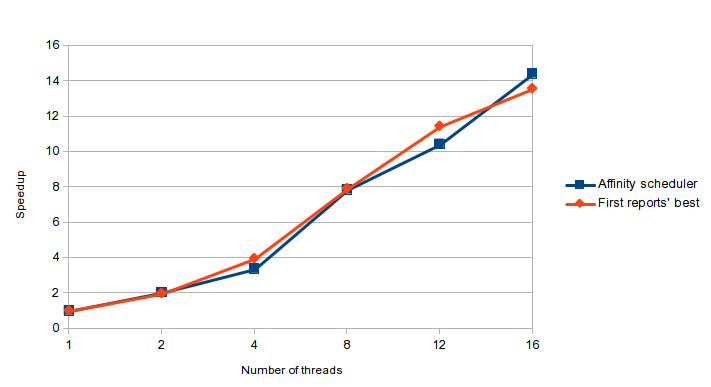
\includegraphics[width=0.95\textwidth]{affinity_vs_best_first.png}
    \caption{Speedup for different schedulers for the first loop.}\label{img:spd_first}
\end{figure}

\begin{figure}[h!]
    \centering
    \includegraphics[width=0.95\textwidth]{time_second.png}
    \caption{Time for different schedulers running the second loop.}\label{img:time_second}
\end{figure}

\begin{figure}[h!]
    \centering
    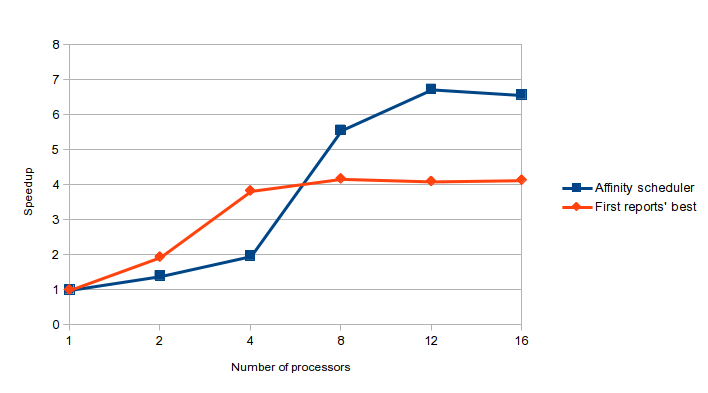
\includegraphics[width=0.95\textwidth]{affinity_vs_best_second.png}
    \caption{Speedup for different schedulers for the second loop.}\label{img:spd_second}
\end{figure}


\newpage
\section{Quick start guide}
In order to build the executable version of the code a relatively recent version of \texttt{OpenMP} is required.
\texttt{GNU Make} is essential, although in its absence it is simple to compile the file too.
In order to compile using the suggested method, execute \texttt{make} from inside the project directory.

Running on a local machine is achieved by simply executing the created \texttt{loops} executable.
If running on \texttt{Morar} or any other machine accepting \texttt{qsub} interface is required, use the provided \texttt{submitter.sh} script runs the executable correctly in such setting.

\end{appendices}

\label{sec:most_loaded}

\end{document}
